

%\documentclass[12pt]{report}

\documentclass[12pt]{article}
%\usepackage{natbib}  % used for citations
\usepackage[parfill]{parskip} %used for formatting style of text



\usepackage{graphicx,fancyhdr}
\usepackage{amssymb,amsmath}
\usepackage{epigraph,fancyvrb,eqparbox}
\usepackage[multiple]{footmisc}
\usepackage{menukeys}
\usepackage{menukeys}
\usepackage{url}
\usepackage[colorlinks = true, linkcolor = blue, urlcolor = blue]{hyperref}
\usepackage{setspace}

\pagestyle{fancyplain}

%\usepackage{hyperref}
%\usepackage{epsf,psfig,graphicx,fancyheadings}
% \textwidth 7in
% \textheight 9in
% \oddsidemargin 0in
% \topmargin -.25in

%-----------------------------------------------
% The following settings are from Dr. Davidian's
% ST810A Handout on Advanced LaTeX Features

%\setlength{\paperheight}{11.0in}
%\setlength{\paperwidth}{8.5in}

%%%%%%%%%%%%%%%%%%%%%%%%%%%%%%%%%%%%%%%%%%%%%%%%%
% For Desktop @ CalPoly (for Postscript)

%\setlength{\oddsidemargin}{0.5in}
%\setlength{\evensidemargin}{0.5in}
%\setlength{\topmargin}{-.5in}

%%%%%%%%%%%%%%%%%%%%%%%%%%%%%%%%%%%%%%%%%%%%%%%%%
% For Laptop @ Calpoly (for Postscript)

% \setlength{\oddsidemargin}{0.in}
% \setlength{\evensidemargin}{0.in}
% \setlength{\topmargin}{0.25in}

%%%%%%%%%%%%%%%%%%%%%%%%%%%%%%%%%%%%%%%%%%%%%%%%%
% For Desktop @ CalPoly (for PDF)

%\setlength{\oddsidemargin}{0.in}
%\setlength{\evensidemargin}{0.in}
%\setlength{\topmargin}{-.5in}
%
%%%%%%%%%%%%%%%%%%%%%%%%%%%%%%%%%%%%%%%%%%%%%%%%%%
%% For Laptop @ Calpoly (for PDF)
%
%% \setlength{\oddsidemargin}{0.in}
%% \setlength{\evensidemargin}{0.in}
%% \setlength{\topmargin}{0.25in}
%
%
%
%\setlength{\oddsidemargin}{0.0in}
%\setlength{\topmargin}{-0.5in}
%\setlength{\headheight}{0.20in}
%\setlength{\headsep}{3ex}
%\setlength{\baselineskip}{2ex}
%\setlength{\textheight}{9in}
%\setlength{\textwidth}{6.4in}
%\renewcommand{\baselinestretch}{1.1}

% Sets margins to 1 in
\addtolength{\oddsidemargin}{-.5in}%
\addtolength{\evensidemargin}{-.5in}%
\addtolength{\textwidth}{1in}%
\addtolength{\textheight}{1.3in}%
\addtolength{\topmargin}{-.8in}%

%\setlength{\headheight}{0.20in}
%\setlength{\headsep}{3ex}
%\setlength{\headrulewidth}{0.2pt}
%\setlength{\footrulewidth}{0.15pt}
%\setlength{\parskip}{2.3ex}
% %set to no indentation
%\setlength{\parindent}{0.0in}
%\setlength{\baselineskip}{2ex}
%\setlength{\textheight}{9.in}
%\setlength{\textwidth}{6.5in}

\def \doublespace{\openup 2\jot}
% For double or 1.5 spacing
%\renewcommand{\baselinestretch}{1.5}
\tolerance=500

\def\boxit#1{\vbox{\hrule\hbox{\vrule\kern6pt
\vbox{\kern6pt#1\kern6pt}\kern6pt\vrule}\hrule}}
\renewcommand{\theequation}{\thesection.\arabic{equation}}
% The following for TOC
%\renewcommand{\thepage}{\roman{page}}
% to be followed by this for the main text
\renewcommand{\thepage}{\arabic{page}}


%-----------------------------------------------

%%%%%%%%%%%%%%%%%%%%%%%%%%%%%%%%%%%%%%
%Define any shortcut aliases below

\newtheorem{theo}{Theorem}[section]

\newenvironment{note}{\begin{quote}\emph{Note:\ }}{\end{quote}}
\newenvironment{defn}{
\begin{description}
\item[Definition ]}
{\end{description}}

\newenvironment{ttscript}[1]{%
    \begin{list}{}{%
    \settowidth{\labelwidth}{\texttt{#1}}
    \setlength{\leftmargin}{\labelwidth}
    \addtolength{\leftmargin}{\labelsep}
    \setlength{\parsep}{0.5ex plus0.2ex minus0.2ex}
    \setlength{\itemsep}{0.3ex}
    \renewcommand{\makelabel}[1]{\texttt{##1\hfill}}}}
    {\end{list}}

\newcommand{\bt}{\begin{tabular}}
\newcommand{\et}{\end{tabular}}
\newcommand{\bc}{\begin{center}}
\newcommand{\ec}{\end{center}}
\newcommand{\bi}{\begin{itemize}}
\newcommand{\ei}{\end{itemize}}
\newcommand{\be}{\begin{enumerate}}
\newcommand{\ee}{\end{enumerate}}
\newcommand{\bq}{\begin{quote}}
\newcommand{\eq}{\end{quote}}
\newcommand{\vect}[1]{\mbox{\boldmath $ #1$}}
\newcommand{\avg}[1]{$\overline{#1}$}
\newcommand{\bmp}{\begin{minipage}}
\newcommand{\emp}{\end{minipage}}
\newcommand{\hr}{\u{\hspace{7in}}}
\newcommand{\sr}{\u{\hspace{5in}}}
\newcommand{\chs}{\chi^2}

\newcommand{\labn}[1]{\Large{\textbf{\fbox{Lab #1}}}\hspace{0.1in} \normalsize{\emph{Some of these problems may be more challenging than others. Please feel free to work with others, attend office hours, or post on the course discussion forum if you need help.  While collaboration with other students is encouraged, each student is responsible for submitting his or her own work.  This assignment should be submitted in one well-commented SAS program.  For any questions that require a written answer, do so in the SAS comments.  Be sure to re-name the uploaded SAS scripts according to the naming convention}} \texttt{LastnameFirstinitial\textunderscore Lab\#.sas} (\emph{e.g.,} \texttt{PileggiS\textunderscore Lab#1.sas}).}


\newcommand{\hd}[1]{\lhead{STAT 330/530: Lab #1}\rhead{Pileggi, FA17}}
\newcommand{\bs}{\underline{\hspace{0.5in}}}

%\newcommand{\bv}{\footnotesize
%\bmp{.5\textwidth}
%\begin{Verbatim}[frame=single,label=SAS Code,commandchars=\\\{\}],xrightmargin=.5\textwidth}
%
%\newcommand{\ev}{\end{Verbatim}
%\emp
%\normalsize}

\newcommand{\bv}{\begin{code}}
\newcommand{\ev}{\end{code}}

 \newenvironment{code}[1]%
  {\vspace{.1in}\footnotesize\Verbatim[frame=single,label=SAS Code,commandchars=\\\{\},xrightmargin=#1\textwidth,framesep=.2in,labelposition=all]}
  {\endVerbatim\normalsize}

\newenvironment{craw}[2]%
{\vspace{.1in}\footnotesize\Verbatim[frame=single,label=#2,commandchars=\\\{\},xrightmargin=#1\textwidth,framesep=.2in,labelposition=all]}
  {\endVerbatim\normalsize}

\newenvironment{cbox}[1]%
{\vspace{.1in}\footnotesize\Verbatim[frame=single,commandchars=\\\{\},xrightmargin=#1\textwidth,framesep=.2in,labelposition=all]}
  {\endVerbatim\normalsize}

\newcommand{\head}[1]{\large \textbf{#1} \normalsize}

\newcommand{\ttt}[1]{\textbf{\texttt{#1}}}


\newcommand{\bsval}[1]{\underline{\hspace{0.2in}{[#1]}\hspace{0.2in}}}

\newcommand{\ttb}{\textbf}
\newcommand{\tte}{\emph}
\newcommand{\ttu}{\underline}



\newcommand{\jdhr}{\vspace{0.2in}\hrule}


\newcommand{\uspace}[1]{\underline{\hspace{#1}}}

\newenvironment{ident}{\begin{list}{}{}
         \item[]}{\end{list}}

\newenvironment{proposition}{
\begin{description}
\item[Proposition: ]}
{\end{description}}

\newcommand{\bpr}{\begin{proposition}}
\newcommand{\epr}{\end{proposition}}



% \newenvironment{example}
%     {
%         \begin{list}{\textbf{Example:}}
%         {
%         \settowidth{\labelwidth}{}
%         \setlength{\leftmargin}{\labelwidth}
%         }
%     }
%     {\end{list}}


\newenvironment{example}{
\jdhr \vspace{-.17in}\jdhr
\textbf{Example: }}
{}

\newcommand{\bex}{\begin{example}}
\newcommand{\eex}{\end{example}}

\newenvironment{onyourown}{
\jdhr \vspace{-.17in}\jdhr
\textbf{On Your Own: }}
{}

\newcommand{\boy}{\begin{onyourown}}
\newcommand{\eoy}{\end{onyourown}}


%\newenvironment{debug}{
%\jdhr \vspace{-.17in}\jdhr
%\ttb{Debug the Code}
%\fbox{
%\bmp{.95in}
%\includegraphics[height=.35in]{C:/images/bug4.jpg}\includegraphics[height=.35in]{C:/images/buggy8.jpg}
%\emp}
%}
%{\jdhr}

\newenvironment{debug}{
\jdhr \vspace{-.17in}\jdhr
\ttb{Debug the Code: }
\fbox{
\bmp{.95in}
\includegraphics[height=.35in]{C:/images/bug4.jpg}\includegraphics[height=.35in]{C:/images/mushi90.jpg}
\emp}
}
{}


\newcommand{\bbug}{\begin{debug}}
\newcommand{\ebug}{\end{debug}}


\begingroup
  \catcode `_=11
  \gdef\myuscore{_}
  \catcode `~=11
  \gdef\mytilde{~}
  \catcode `\|=0
  \catcode `\\=11
  |gdef|mybs{\}
|endgroup

%Define any shortcut aliases above


%....................................................................
%....................................................................
%....................................................................
%....................................................................
%....................................................................
%....................................................................
%....................................................................
%....................................................................



\usepackage{amssymb}
				




\begin{document}
\hd{3}
\labn{3}
\vskip10pt
The \texttt{mariokart} data set includes all auctions on Ebay for a full week in October, 2009. Auctions were included in the data set if they satisfied a number of conditions. (1) They were included in a search for "wii mario kart" on ebay.com, (2) items were in the Video Games $>$ Games $>$ Nintendo Wii section of Ebay, (3) the listing was an auction and not exclusively a ``Buy it Now'' listing (sellers sometimes offer an optional higher price for a buyer to end bidding and win the auction immediately, which is an optional Buy it Now auction), (4) the item listed was the actual game, (5) the item was being sold from the US, (6) the item had at least one bidder, (7) there were no other items included in the auction with the exception of racing wheels, either generic or brand-name being acceptable, and (8) the auction did not end with a Buy It Now option.  All prices are in US dollars. Our goal for this lab to create models for the total selling price of the Ebay package (\ttt{totalPr}).
\vskip10pt
\ttt{mariokart.sas7bdat}:\\
\vskip5pt
\begin{tabular}{r|l}
\ttt{ID} &   	Auction ID assigned by Ebay.\\
\ttt{duration} & 	Auction length, in days. \\
\ttt{nBids} &		Number of bids.	 \\
\ttt{cond} & 		Game condition, either new or used. \\
\ttt{startPr} &	Starting price of the auction. \\
\ttt{shipPr} &	Shipping price. \\
\ttt{totalPr} &	Total price, which equals the auction price plus the shipping price. \\
\ttt{shipSp} & 	Shipping speed or method. \\
\ttt{sellerRate} & 	The seller's rating on Ebay (number of positive ratings minus the \\
& number of negative ratings). \\
\ttt{stockPhoto} &	Whether or not the auction feature photo was a ``stock'' photo. \\
\ttt{wheels} &	Number of Wii wheels included in the auction. \\
\ttt{title} &		The title of the auctions. \\
\end{tabular}
\vskip10pt
\begin{enumerate}
\item Identify the \ttt{mariokart.sas7bdat} file from either PolyLearn or the shared drive.  Save the file to a location on your computer or your flash drive.
\item Create a library reference called \texttt{mylib} to access the \ttt{mariokart.sas7bdat}.
\item Explore the \emph{total selling price} variable with any of PROCS that we have learned so far (\texttt{PROC CONTENTS, PROC PRINT, PROC MEANS, PROC FREQ, PROC UNIVARIATE}).  There are a two observations that really don't fit the pattern of the rest with regards to total selling price.  Identify these observations and explain why they are outliers in a comment in your SAS code.  (In future classes we will learn how to ``clean'' these observations, but for now we will leave them as is.)
\item An eBay official claims that the population mean number of bids received exceeds 10.  Test the hypotheses $H_0$: $\mu=12$ vs $H_a$: $\mu \neq 12$ and compute a 95\% confidence interval for $\mu$ using \texttt{PROC UNIVARIATE}.  Fill in the blanks in the paragraph below to interpret the results.
\begin{itemize}
\item[] \doublespacing
        Based on \underline{(insert \#)} packages for sale on eBay, the average number of bids a package received is \bs with a standard deviation of \bs.  We used a one sample t-test to test $H_0$: $\mu=12$ vs $H_a$: $\mu \neq 12$, where $\mu$ represents the population average number of bids.  The test statistic is $t=$ \bs and the $p$-value is \bs.  We \underline{(do / do not)} have evidence that the population mean number of bids differs from 12.  Furthermore, a 95\% confidence interval for the population mean number of bids is (\bs, \bs).  This \underline{(does / does not)} provide evidence that the population mean number of bids exceeds 12.
\end{itemize} 
\item Replicate your summary statistics and confidence interval findings (not the hypothesis test) from the previous question using \ttt{PROC MEANS}.  Below is the output that you are trying to achieve.  \emph{Hint: you need to use statistics key words.}
\item[] \bmp{.5\textwidth}
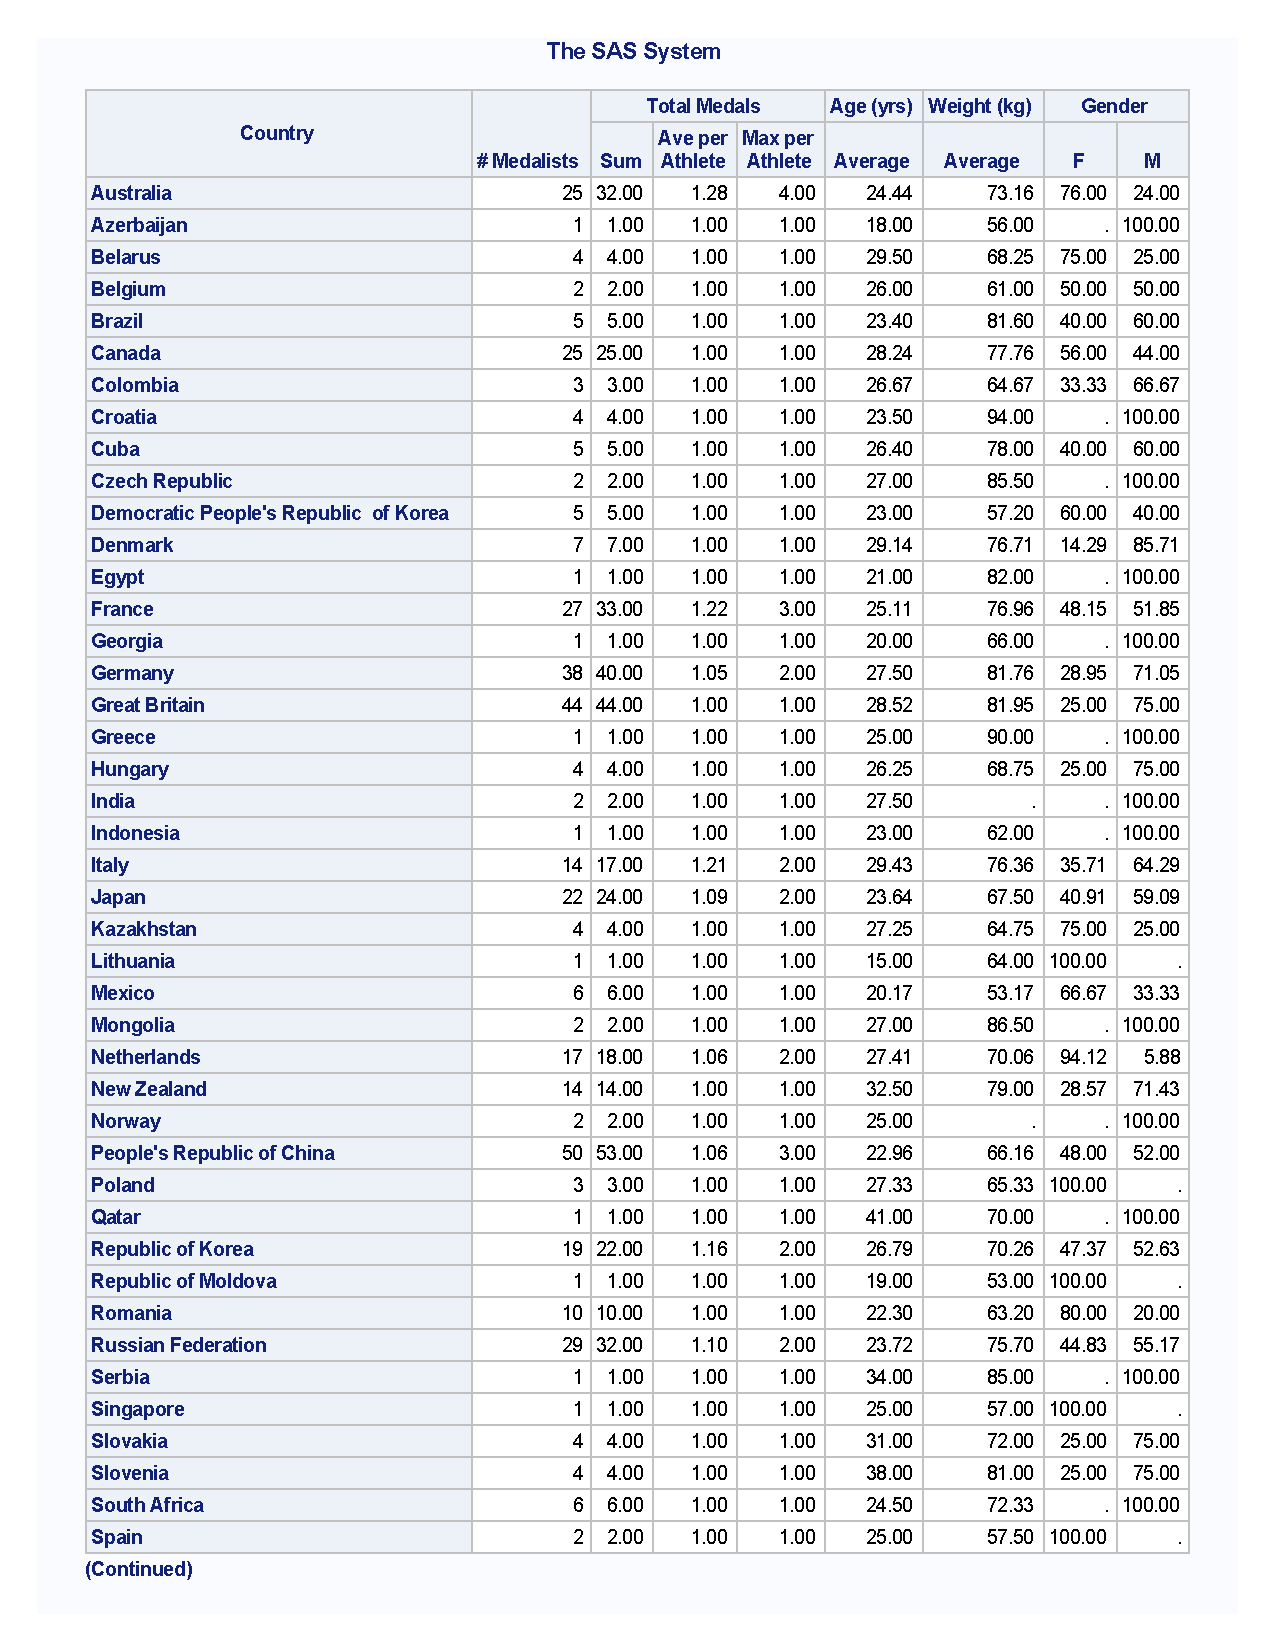
\includegraphics[trim={5cm 23cm 5cm 0cm},clip]{q5.pdf}
\emp
\item Use a SAS procedure to identify the percent of packages that were sold with 2 wheels.  Note your findings as a comment in your SAS code.
\item Examine the relationship between condition of the package and number of wheels by creating a contingency table with wheels on the rows and condition on the columns.  In a comment in your SAS code, report the percent of new packages that came with zero wheels and the percent of used packages that came with zero wheels.  Modify your table so that only frequencies and these percents are presented.  \emph{(Your table will still be 4x2, with total rows and columns, but each cell should only have two numbers: a frequency and the relevant percent to compare new versus used packages.)}
\item Perform a chi-squared test to determine if there is an association between condition of the package and whether or not the package has a stock photo; in addition, print the expected cell counts for the table.  (\emph{Hint: Use the help file, this is an option on the TABLES statement.}) The contingency table should only display frequencies and expected cell counts, as shown in the output below.  Fill in the blanks in the following paragraph to interpret the results.
\begin{itemize}
\item[] \doublespacing
        We used a chi-squared test to assess $H_0$: there \underline{(is / is not)} an association between condition and stock photo versus $H_a$: there \underline{(is / is not)} an association between condition and stock photo.  The chi-squared test statistic is $\chi^2=$ \bs and the $p$-value is \bs.  We \underline{(do / do not)} have evidence of an association between condition of the package and stock photo.  Furthermore, \underline{\emph{(insert \#)}} expected cell counts exceed 5, so the expected cell count condition for the chi-squared test \underline{(is / is not)} satisfied.
\end{itemize} 
\item[] \bmp{.5\textwidth}
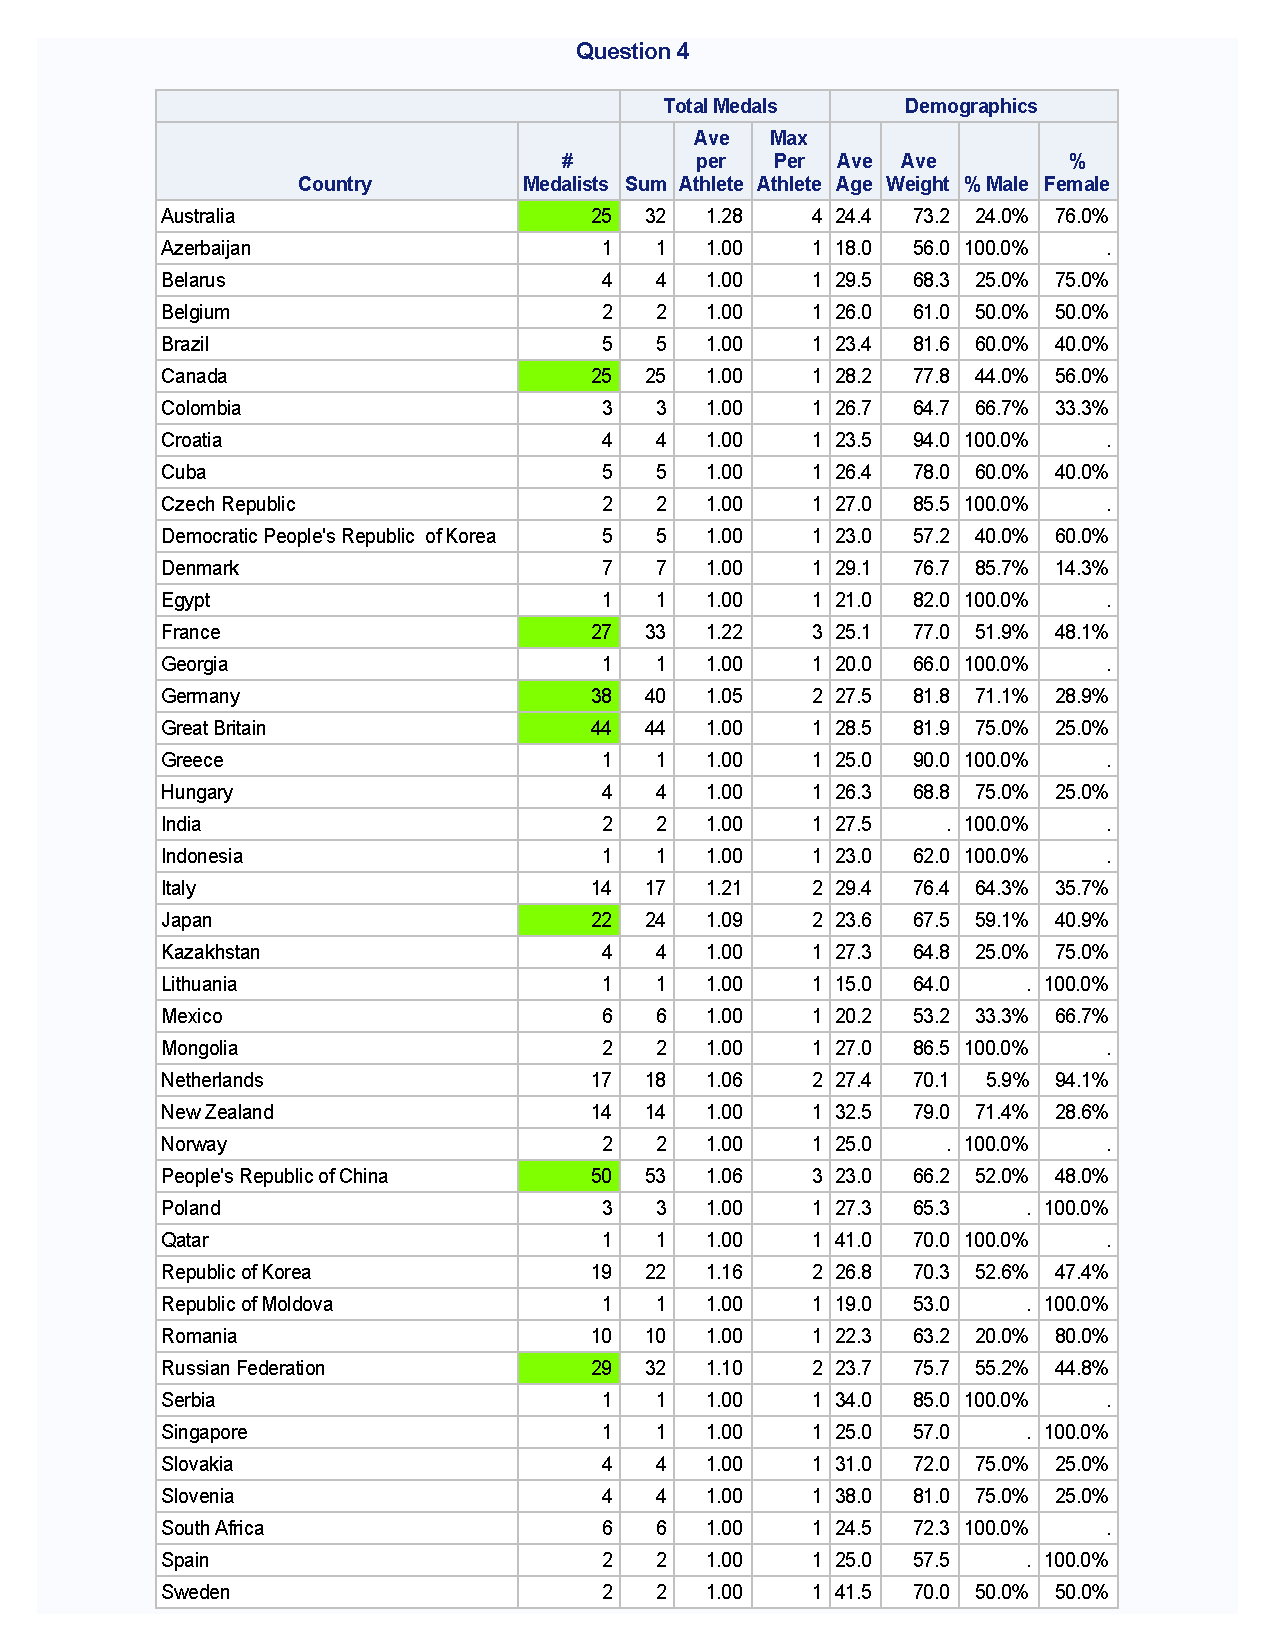
\includegraphics[trim={4cm 10cm 4cm 0cm},clip]{q8.pdf}
\emp
\end{enumerate}

\end{document}